\documentclass[a4paper, 12pt, twoside, openright]{article}
\usepackage[T1]{polski}
\usepackage[utf8]{inputenc}
\newtheorem{theorem}{Twierdzenie}
\usepackage{helvet}
\usepackage{graphicx}
\usepackage{color}
\usepackage{subfig}
\usepackage[table, svgnames, dvipsnames]{xcolor} 
\usepackage{array}
\usepackage{float}
\usepackage{cellspace}
\usepackage[top=1.3in,bottom=1.3in,right=1in,left=1in,headheight=95pt,headsep=-0.5cm]{geometry}
\usepackage{color}
\usepackage{listings}
\usepackage{caption}
\usepackage{cmap}

\usepackage{enumitem}
\setlist{nolistsep}
\usepackage{hyperref}



\newcounter{nalg} 
\DeclareCaptionLabelFormat{algocaption}{Algorytm \thenalg}
\lstnewenvironment{algorithm}[1][] 
{   
	\refstepcounter{nalg}
	\captionsetup{labelformat=algocaption,labelsep=colon} 
	\lstset{ 
		mathescape=true,
		frame=tB,
		numbers=left, 
		numberstyle=\tiny,
		basicstyle=\scriptsize, 
		keywordstyle=\color{black}\bfseries\em,
		keywords={,input, def, output, return, datatype, function, in, if, else, foreach, while, begin, end }
		numbers=left,
		xleftmargin=.04\textwidth,
		#1 
	}
}
{}



\begin{document}

\lstset{language=Python}
% =====  STRONA TYTULOWA  ====

\thispagestyle{empty}
\vspace*{-0.6in}
%% ------------------------ NAGLOWEK STRONY =======================------

\includegraphics[height=37.5mm]{img/logo_agh}\\
\rule{30mm}{0pt}
{\large\textsf{Wydział Fizyki i Informatyki Stosowanej}}\\
\rule{\textwidth}{3pt}\\
\rule[2ex]
{\textwidth}{1pt}\\
\vspace{3ex}
\begin{center}
{\bf\LARGE\textsf{Praca inżynierska}}\\
\vspace{13ex}
% ======================= IMIE I NAZWISKO =======================----
{\bf\Large\textsf{Patryk Chodur}}\\
\vspace{3ex}
{\sf \small kierunek studiów:} {\bf\small\textsf{informatyka stosowana}}\\
\vspace{15ex}
%% ------------------------ TYTUL PRACY --------------------------------------
{\bf\huge\textsf{Opracowanie wtyczki do dekodowania
	pakietów Ethernet z~wykorzystaniem oprogramowania Wireshark
}}\\
\vspace{14ex}
%% ------------------------ OPIEKUN PRACY ------------------------------------
{\sf \Large Opiekun:} {\bf\Large\textsf{dr hab. inż. Bartosz Mindur}}\\
\vspace{22ex}
\textsf{\bf\large\textsf{Kraków, styczeń 2021}}
\end{center}


\newpage

%% =====  Oświadczenie =========
\begin{center}
	{\bf\large\textsf{Oświadczenie studenta}}
\end{center}


{\sf Uprzedzony(-a) o odpowiedzialności karnej na podstawie art. 115 ust. 1 i 2 ustawy z dnia 4 lutego 1994 r. o prawie autorskim i prawach pokrewnych (t.j. Dz. U. z 2018 r. poz. 1191 z późn. zm.): „Kto przywłaszcza sobie autorstwo albo wprowadza w błąd co do autorstwa całości lub części cudzego utworu albo artystycznego wykonania, podlega grzywnie, karze  ograniczenia wolności albo pozbawienia wolności do lat 3. Tej samej karze podlega, kto rozpowszechnia bez podania nazwiska lub pseudonimu twórcy cudzy utwór w wersji oryginalnej albo w postaci opracowania, artystyczne wykonanie albo publicznie zniekształca taki utwór, artystyczne wykonanie, fonogram, wideogram lub nadanie.”, a także uprzedzony(-a) o odpowiedzialności dyscyplinarnej na podstawie art. 307 ust. 1 ustawy z dnia 20 lipca 2018 r. Prawo o szkolnictwie wyższym i nauce (Dz. U. z 2018 r. poz. 1668 z późn. zm.) „Student podlega odpowiedzialności dyscyplinarnej za naruszenie przepisów obowiązujących w uczelni oraz za czyn uchybiający godności studenta.”, oświadczam, że niniejszą pracę dyplomową wykonałem(-am) osobiście i samodzielnie i nie korzystałem(-am) ze źródeł innych niż wymienione w pracy

\bigskip

Jednocześnie Uczelnia informuje, że zgodnie z art. 15a ww. ustawy o prawie autorskim i prawach pokrewnych Uczelni przysługuje pierwszeństwo w opublikowaniu pracy dyplomowej studenta. Jeżeli Uczelnia nie opublikowała pracy dyplomowej w terminie 6 miesięcy od dnia jej obrony, autor może ją opublikować, chyba że praca jest częścią utworu zbiorowego. Ponadto Uczelnia jako podmiot, o którym mowa w art. 7 ust. 1 pkt 1 ustawy z dnia 20 lipca 2018 r. — Prawo o szkolnictwie wyższym i nauce (Dz. U. z 2018 r. poz. 1668 z późn. zm.), może korzystać bez wynagrodzenia i bez konieczności uzyskania zgody autora z utworu stworzonego przez studenta w wyniku wykonywania obowiązków związanych z odbywaniem studiów, udostępniać utwór ministrowi właściwemu do spraw szkolnictwa wyższego i nauki oraz korzystać z utworów znajdujących się w prowadzonych przez niego bazach danych, w celu sprawdzania z wykorzystaniem systemu antyplagiatowego. Minister właściwy do spraw szkolnictwa wyższego i nauki może korzystać z prac dyplomowych znajdujących się w prowadzonych przez niego bazach danych w zakresie niezbędnym do zapewnienia prawidłowego utrzymania i rozwoju tych baz oraz współpracujących z nimi systemów informatycznych.}

\vspace{14ex}

\begin{center}

~~~~~~~~~~~~~~~~~~~~~~~~~~~~~~~~~~~~~~~~~~~~~~~~~~~~~~~~~~~~~~~~~ 
................................................................. \\
~~~~~~~~~~~~~~~~~~~~~~~~~~~~~~~~~~~~~~~~~~~~~~~~~~~~~~~~~~~~~~~  {\sf (czytelny podpis)} \\

\end{center}

%% =====  TYL STRONY TYTULOWEJ   ====


%% ============ OCENA OPIEKUNA =============
\newpage
\linespread{1.3}
\selectfont

\hspace*{\fill}\large{Ocena merytoryczna opiekuna}

\vspace{85mm}

%% ============ OCENA RECENZENTA =============
\newpage
\linespread{1.3}
\selectfont

\hspace*{\fill}\large{Ocena merytoryczna recenzenta}

\vspace{85mm}


%% ====== SPIS TRESCI ==========
\newpage
\tableofcontents


%=======================- 1 =======================
\newpage
\section{Wstęp}
\subsection{Wprowadzenie}
	\indent\par
	Wireshark jest oprogramowaniem do analizy ruchu internetowego na poziomie pakietów wydanym na otwartej licencji GPL2.
	Jednym z jego podstawowych funkcjonalności jest podglądanie zawartości przechodzących przez łącze internetowe danych.
	Dokonuje się go za pomocą dekoderów (ang. dissector). Dekodery mają strukturę hierarchiczną - wyjście jednego
	może stanowić wejście drugiego dekodera.

	\begin{figure}[h]
		\centering
			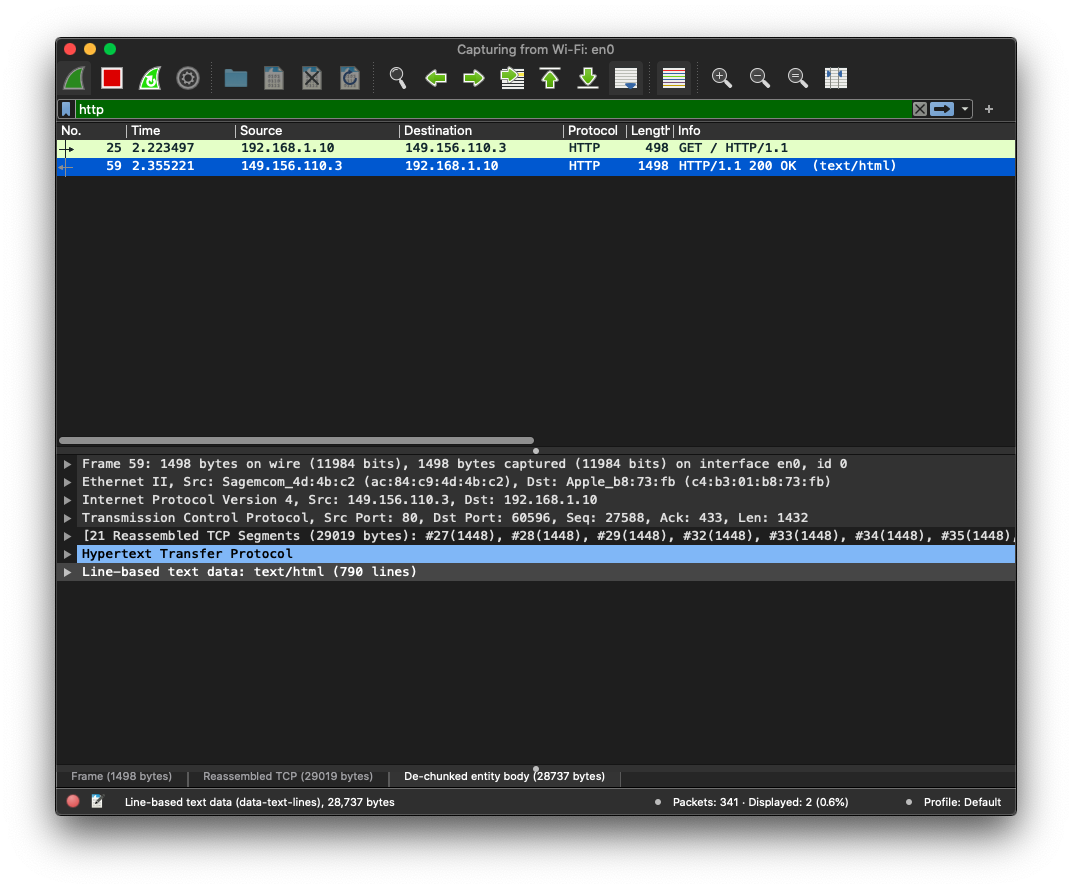
\includegraphics[width=1.0\textwidth]{img/screenshot_fis.png}
		\caption{Przykładowa struktura pakietu http po wyświetleniu w przeglądarce strony http://www.fis.agh.edu.pl}
		\label{fig:fis}
	\end{figure}

	Na powyższym rysunku (Rys.~\ref{fig:fis}) widać kolejne poziomy dekodowania pakietu http. Są to:
	\begin{itemize}
		\item Interfejs en0
		\item Protokół Ethernet
		\item Protokół IPv4
		\item Protokół TCP
		\item Dodatkowy poziom złożonych pakietów TCP
		\item Protokół http
		\item Dane tekstowe
	\end{itemize}

	Każdy dekoder jest osobnym modułem, dzięki czemu np. dekoder http może czytać także dane idące protokołem UDP.
	Dekodery rejestrują zainteresowanie danymi pakietami dekoderowi wyżej w hierarchii, więc dekoder http może przykładowo
	żądać danych przesyłanych protokołem TCP na porcie 80.

	Głównym zadaniem dekoderów jest wyświetlanie przesyłanych informacji w sposób zrozumiały dla użytkownika. Za pomocą
	interfejsu graficznego wyświetlają one zinterpretowane przez siebie dane transmisji. Sposób przedstawienia danych
	jest arbitralną decyzją programisty, więc podstawowymi kryteriami podczas projektowania są użyteczność oraz czytelność.

	\begin{figure}[h]
		\centering
			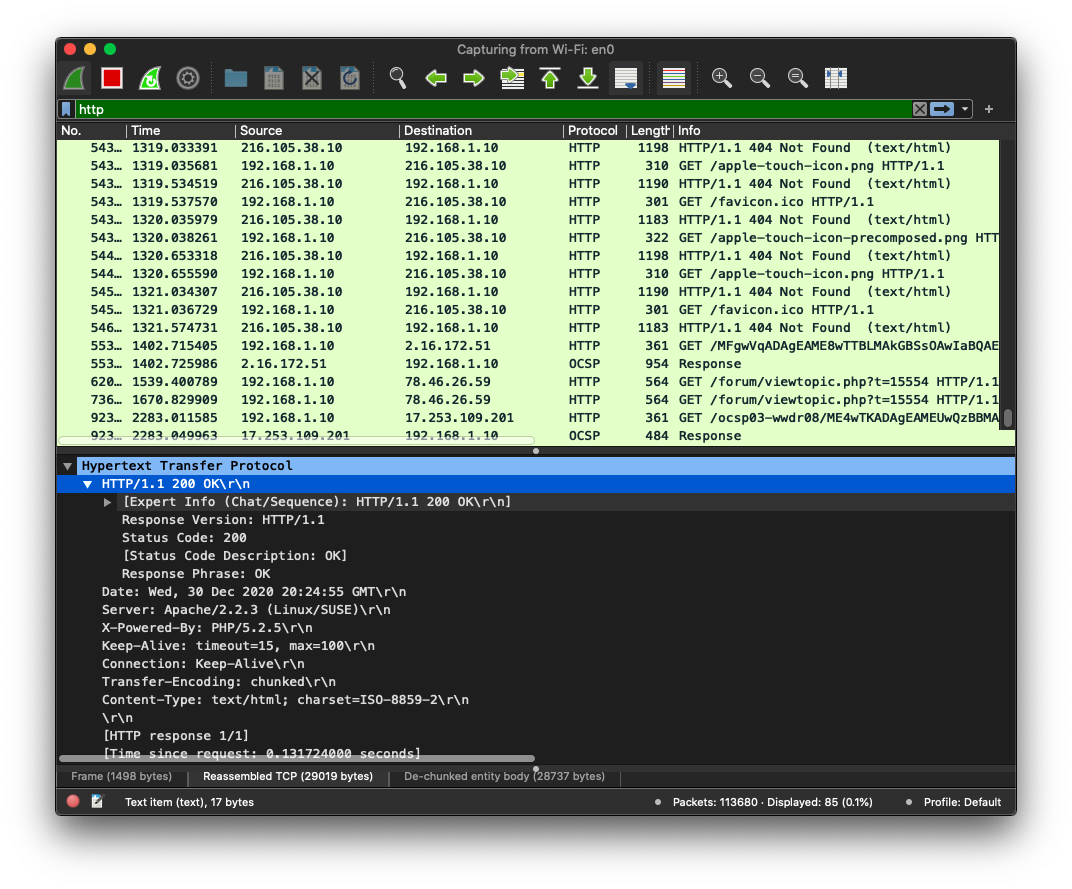
\includegraphics[width=1.0\textwidth]{img/screenshot_fis_http.png}
		\caption{Binarne dane protokołu http zinterpretowane przez odpowiedni dekoder i wyświetlone w oknie programu.}
		\label{fig:fis_http}
	\end{figure}

\newpage

\subsubsection{Tworzenie dekoderów}

	\indent\par
	Program Wireshark wyposażony jest w zestaw dekoderów do najczęściej wykorzystywanych protokołów. Twórcy programu
	dają jednakże możliwość tworzenia własnych. Głównym celem ich tworzenia jest możliwość
	dekodowania własnych protokołów oraz reintepretacja już istniejących. Dostępne są trzy sposoby ich pisania:
	\begin{itemize}
		\item Tekstowe - opisana w formie tekstowej struktura pakietu oraz inne, konieczne do zdekodowania informacje.
		\item Skryptowe - dekoder napisany w języku skryptowym, np. \texttt{lua} czy \texttt{python}
		\item Kompilowane, w języku C - dekoder napisany jako kompilowana wtyczka w C
	\end{itemize}

	Tekstowe dekodery są najprostsze w implementacji, jednak działają zwykle najwolniej, a ich możliwości są ograniczone.
	Dekodery napisane w C mają największe możliwości, gdyż mogą chociażby korzystać z \texttt{libwireshark}. Działają zwykle
	najszybciej, a gotowy plugin łatwo jest przenieść do innej instalacji, ale ich problemem jest wyższy próg wejścia. 
	Są też najobszerniejsze i najmniej czytelne.

	Kompromis pomiędzy tymi dwoma podejściami stanowi pisanie w języku skryptowym. Najczęściej wykorzystywany w tym celu jest
	język \texttt{lua}. Cieszy się on wbudowanym wsparciem ze strony programu Wireshark oraz stosunkowo dużą społecznością.



\subsection{Cel pracy}

	\indent\par
	Celem pracy jest wykonanie dekodera pakietów bazujących na protokole UDP i~przenoszących konkretne dane pomiarowe.
	Dekoder napisany jest jako wtyczka do programu Wireshark. Podejście takie umożliwia szybszą rekompilację wtyczki,
	niewymagającą przekomilowywania całego programu, a~także użycie gotowej wtyczki z~dowolną instalacją programu Wireshark,
	o~ile zachowana jest zgodność systemu operacyjnego i~wersji programu Wireshark. Instalacja polega na przekopiowaniu
	pojedyńczego pliku do katalogu wtyczek programu. Alternatywą dla takiego rozwiązania jest stworzenie wbudowanego dekodera,
	ale ze względu na liczne wady - m.~in.: dłuższy czas rekompilacji oraz konieczność ingerencji w~kod źródłowy programu - rozwiązanie
	to nie zostało zastosowane.


\newpage
\section{Narzędzia}
\subsection{Kod źródłowy}

	\indent\par
	Wtyczka napisana została w języku C, bez jawnego użycia zewnętrznych bibliotek. Wykorzystane pliki nagłówkowe
	pochodzą ze standardowej biblioteki C, oraz kodu źródłowego programu Wireshark. Program Wireshark używa wielu
	bibliotek, takich jak qt oraz gthread, ale na wyszczególnienie zasługuje biblioteka glib w wersji drugiej, której
	elementy zostały użyte w kodzie źródłowym aplikacji. Glib2 dostarcza projektowi standardowych typów o stałym
	rozmiarze wykorzystywanych przez niektóre funkcje Wireshark.
	
	Cały kodu projektu napisany został w programie Vim.

\subsection{Kompilacja}

	\indent\par
	Podczas kompilacji projektu wykorzystywane jest narzędzie cmake. Służy ono do zarządzania procesem kompilacji,
	umożliwiając jednolity proces budowy projektu
	na każdym ze wspieranych systemów operacyjnych. Wykrywa ono konieczne do zbudowania narzędzia, informując
	o brakujących, a także, w zależności od systemu operacyjnego, tworzy skrypty kompilacyjne. Na systemach Unixowych
	oznacza to zwykle generowanie plików Makefile, na systemie Windows - projektu w Visual Studio. Użycie cmake'a
	jest pierwszym krokiem standardowej kompilacji programu Wireshark oraz jego wtyczek.
	
	Do kompilacji wymagany jest kompilator do języka C. Decyzję o wykorzystaniu konkretnego narzędzia podejmuje cmake.
	W razie braku stosownego kompilatora cmake poinformuje użytkownika o problemie. Ponadto wymagany jest szereg
	bibliotek.

	\newpage

	Część wymagnych bilbiotek dla Wireshark 3.4.2:
	\begin{itemize}
		\item \texttt{GLIB2} - biblioteka od GNU będąca implementacją biblioteki standardowej C wraz z wieloma rozszerzeniami.
		\item \texttt{GTHREAD2} - biblioteka do wielowątkowości od GNU.
		\item \texttt{GCRYPT} - bibliokeka kryptograficzna od GNU.
		\item \texttt{CARES} - bilbioteka do asynchronicznych zapytań DNS.
		\item \texttt{LEX} - generator analizatorów leksykalnych. Najczęściej flex.
		\item \texttt{YACC} - generatoror analizatorów składniowych. Najczęściej bison.
		\item \texttt{Perl} - interpreter oraz zestaw narzędzi do języka perl.
		\item \texttt{Python3} - interpreter oraz zestaw narzędzi do języka python w wersji 3.
		\item \texttt{M} - biblioteka do obliczeń matematycznych będąca częścią biblioteki standardowej C.
		\item \texttt{Qt5} - biblioteka do budowania przenośnych interfejsów graficznych.
	\end{itemize}

	\indent\par
	Podczas tworzenia wtyczki wykorzystane zostały dwa proste narzędzia napisane przez autora pracy:
	\begin{itemize}
		\item \texttt{printhex} - program napisany w C służący do wyświetlania otrzymanych bajtów w zapisie szesnastkowym. Standardowo
			czyta on z stdin i wysyła output na stdout, lecz możliwe jest podanie nazwy plików wejściowego oraz wyjściowego.
		\item \texttt{reverse} - program zamieniający kolejność bitów w masce - np \texttt{0xFCull} na \texttt{0x3F00000000000000ull}.
			Nie posiada on żadnych dodatkowych funkcjonalności i czyta ze stdin.
	\end{itemize}




\newpage
\section{Implementacja}
\subsection{Plugin w C}
Dekoder został zaimplementowany jako plugin w języku C. 
\subsubsection{Struktura programu}

\subsection{CMake}

\subsection{}


\newpage
\bibliographystyle{srt}
\begin{thebibliography}{99}

	\bibitem{WGDS}
		http://wsgd.free.fr [dostęp: 30.12.2020]


\end{thebibliography}


\vspace{85mm}


\end{document}

